\subsection{Definição dos modelos genéricos}
Com base no INI-C (2018) e no levantamento das edificações de escritório de Vitória, foram 
propostos dois tipos de modelos genéricos como base para o estudo das modificações de 
otimização e de produção de energia. Estes modelos representam os dois cenários de ambiente 
construído mais observados na cidade de Vitória. Estes cenários são formados por edificações 
mais baixas, com 8 pavimentos, e as mais altas, com 19 pavimentos. As dimensões utilizadas 
como referência para a construção dos modelos genéricos foram resultado dos valores médios 
observados nas edificações que compõe o levantamento.\vspace*{0.3cm} \newline
As características predominantes aplicadas aos modelos genéricos foram:
    \begin{itemize}
        \item Número de pavimentos;
        \item Forma - retangular;
        \item Altura - gabarito e dimensões das fachadas;
        \item Layout interno dos pavimento-tipo;
        \item Ausência de proteção solar;
        \item Percentual Total de Área de Abertura da Fachada.
    \end{itemize}
A composição dos modelos é baseada nas características predominantes e nos dados coletados 
\textit{in site}.
\subsubsection{Composição dos modelos genéricos}
A composição construtiva atribuída aos modelos utilizados neste trabalho mostra fundamentalmente 
os parâmetros necessários para a avaliação do desempenho energético segundo o INI-C. Os 
atributos utilizados serviram como ponto de partida para as análises subsequentes sugeridas nas 
etapas metodológicas e estão dispostos no Fluxograma da Figura \ref{fig:figura8}.\vspace*{0.3cm}

    \begin{figure}[ht]
        \centering
        \caption{\small Fatores utilizados como parâmetros de configuração volumétrica dos modelos genéricos.}
        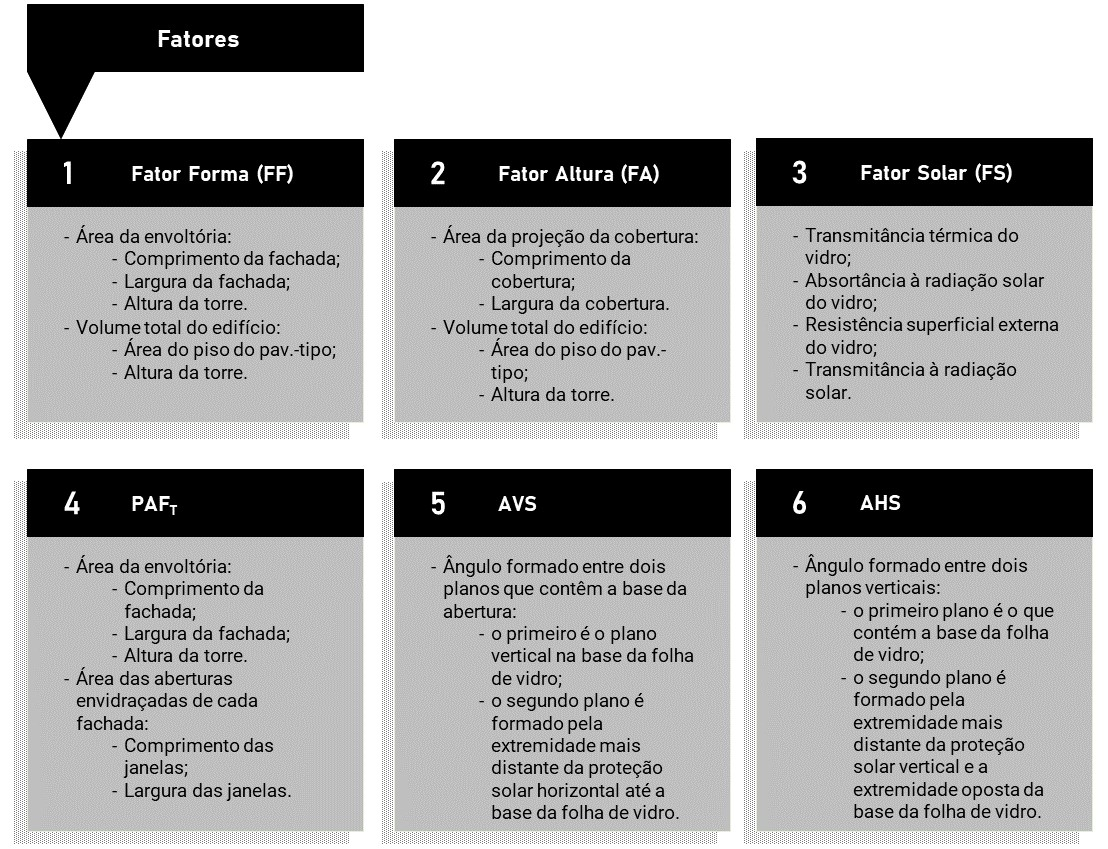
\includegraphics[width=0.8\textwidth]{figures/fig10_Fluxogramas-2.jpg}
        \begin{flushleft}
            \par \small Fonte: autor (2019)
        \end{flushleft}
        \label{fig:figura8}
    \end{figure}

\noindent Apresentados na Tabela 7 e exemplificado na Figura \ref{fig:figura9}, os atributos estudados foram Fator de 
Forma, FF, Fator Altura, FA, Percentual de Área de Abertura da Fachada Total, PAFT, Ângulo 
Vertical de Sombreamento, AVS, e Ângulo Horizontal de Sombreamento, AHS.
    \begin{figure}[ht]
        \centering
        \caption{\small Estrutura arquitetônica dos modelos genéricos.}
        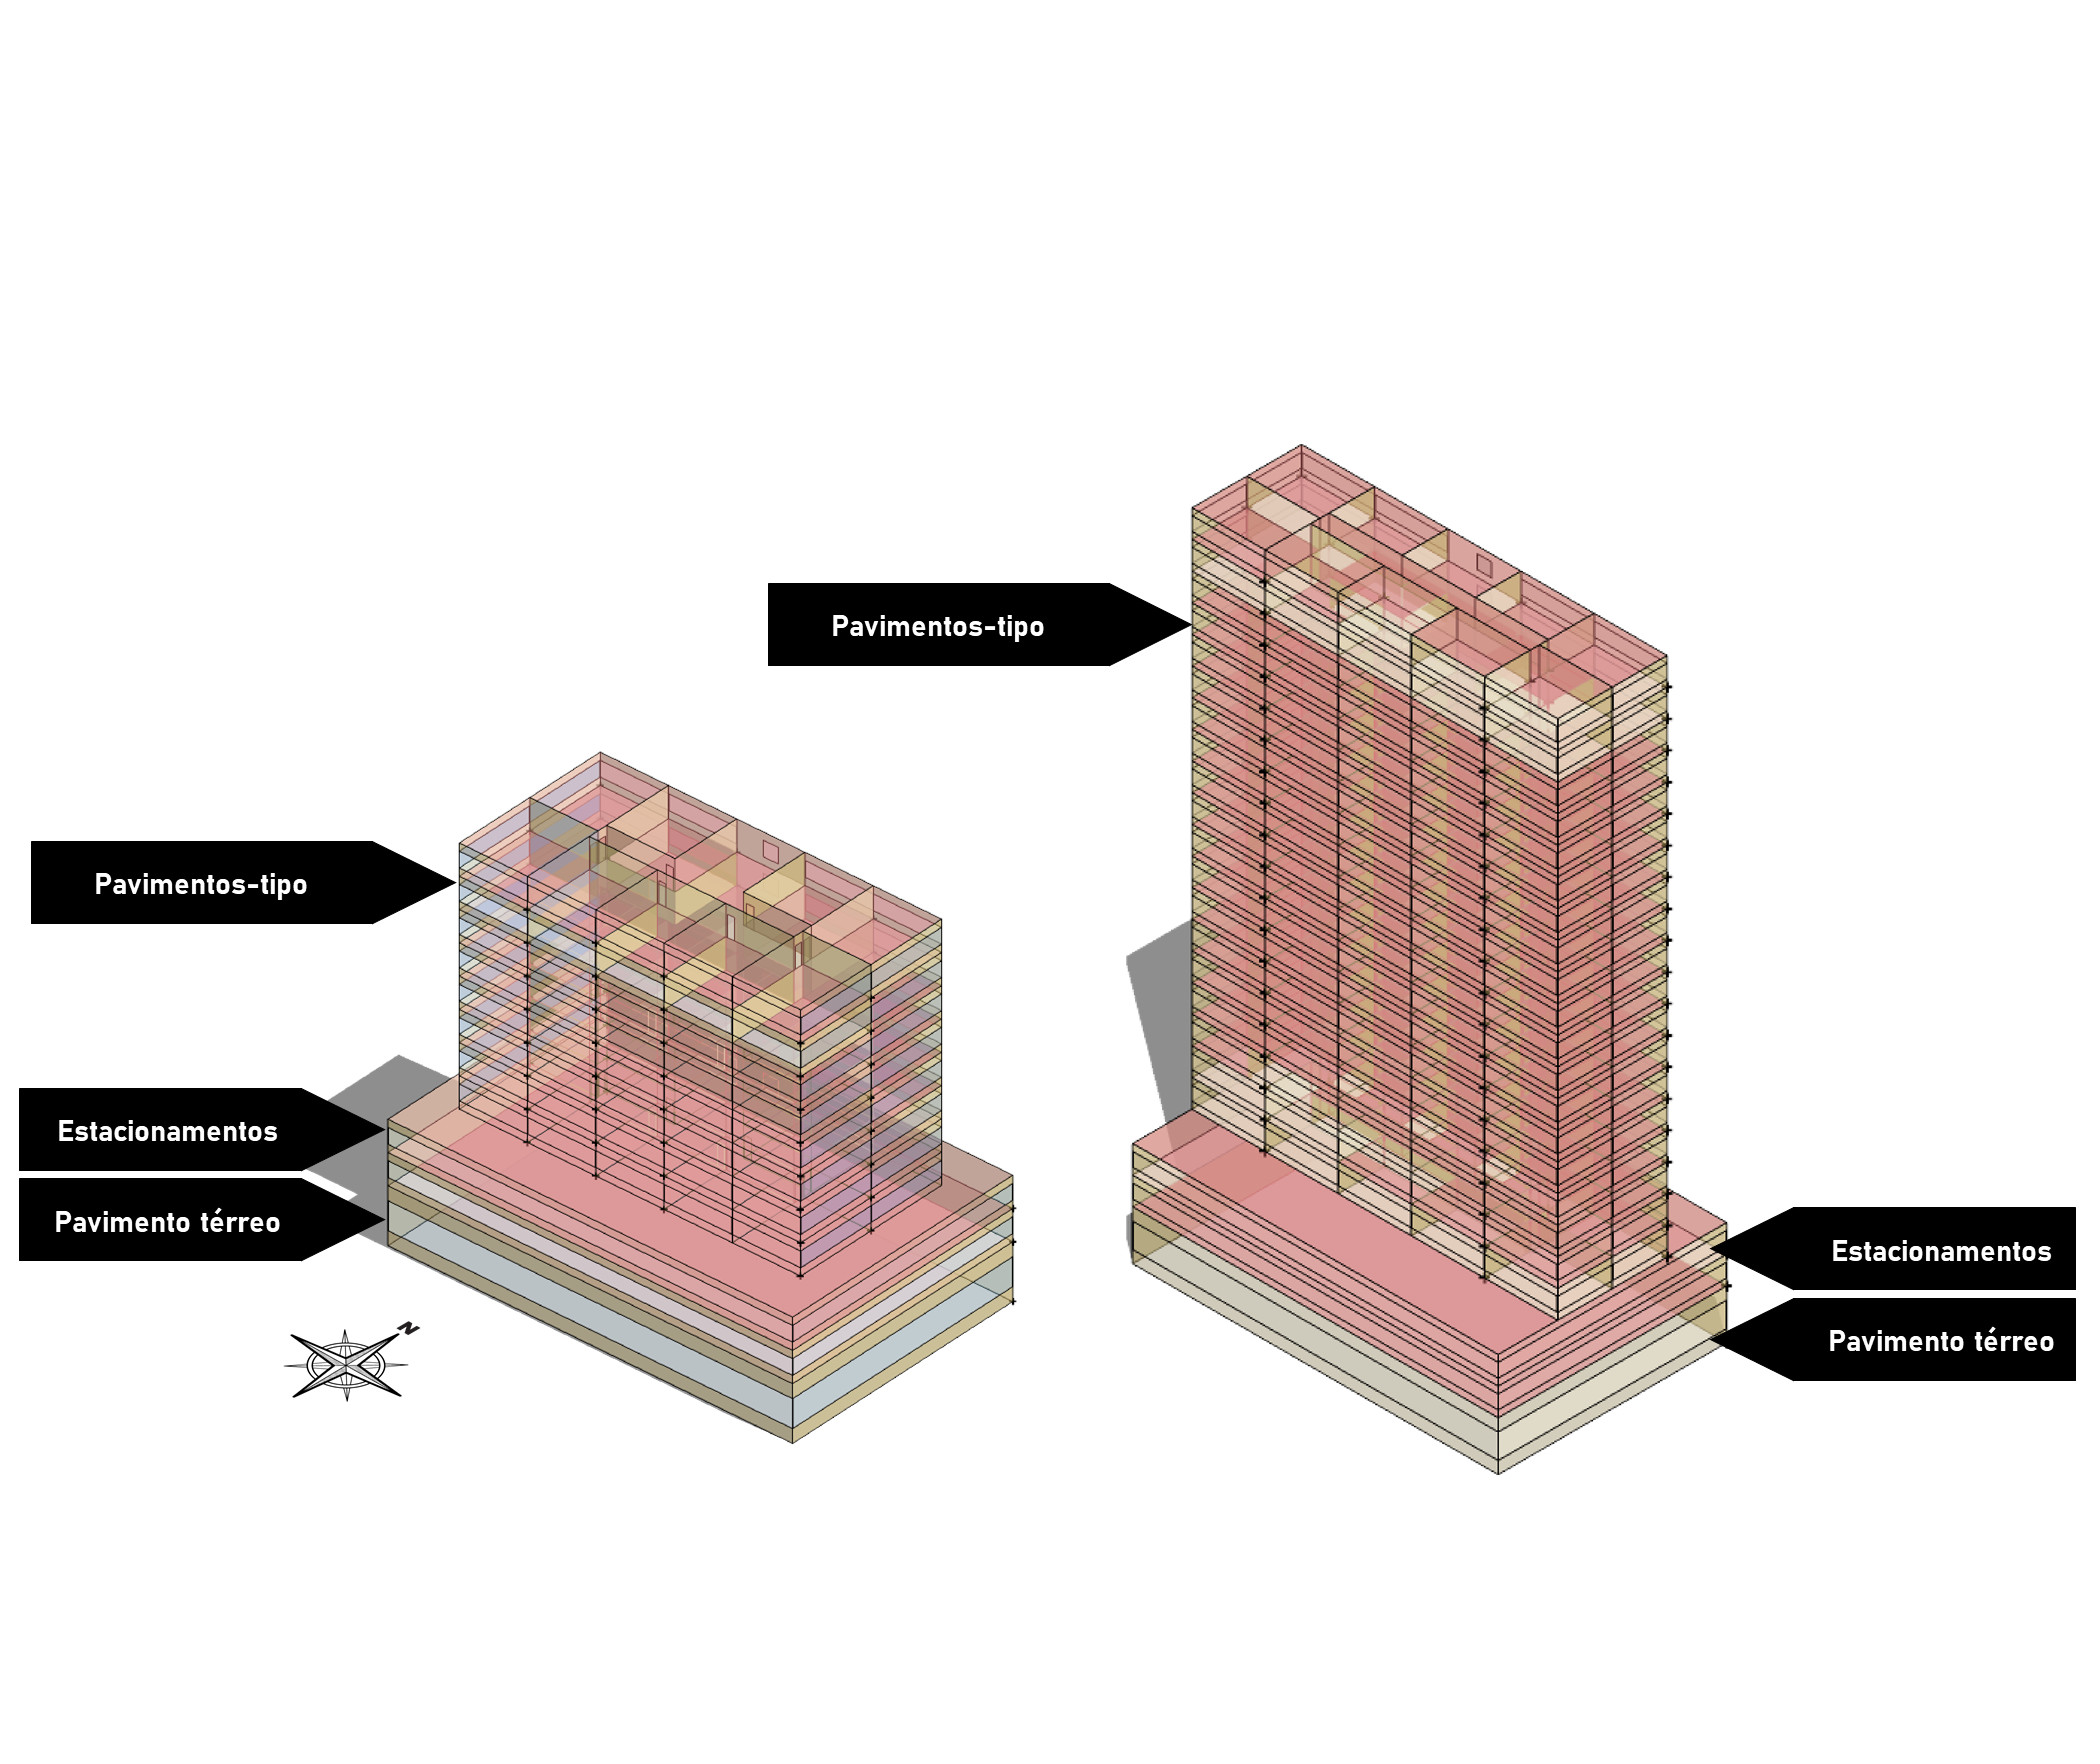
\includegraphics[width=0.1\textwidth]{figures/fig11_8-19-2pav.png}
        \begin{flushleft}
            \par \small Fonte: autor (2019).
        \end{flushleft}
        \label{fig:figura9}
    \end{figure}\newline
\noindent O PAFT e as propriedades do vidro utilizados para os modelos genéricos, como Fator Solar – FS, 
ou Solar Heat Gain Coefficient – SHGC, foram adotados considerando as médias desses atributos 
coletados in loco e complementados por dados extraídos do Catálogo de Propriedades Térmicas e 
Óticas de Vidro \cite{CentroBrasileirodeEficienciaEnergeticaemEdificacoesCB3E2015,AssociacaoBrasileiradeNormasTecnicas-ABNT2003}, da NBR 15220 (2003) e do INI-C \cite{InstitutoNacionaldeMetrologiaNormalizacaoeQualidadeIndustrial-INMETRO2018}, 
como forma de tornar genéricos os dados empregados, como apresentado na Tabela \ref{tab:tabela8}.\vspace*{0.3cm} \newline
\begin{table}[ht]\centering
    \caption{\small Parâmetros arquitetônicos dos modelos genéricos.}
    \vspace*{0.3cm}
    \label{tab:tabela8}
    \begin{tabular*}{\columnwidth}{@{\extracolsep{\fill}}l|ll}
    \hline
    \textbf{Parâmetro}                                                              & \textbf{Descrição}         & \textbf{Referências}  \\ \hline
    \multicolumn{3}{c}{\textbf{Dados dimensionais dos pavimentos-tipo}}\\\hline
    Número de pavimento (un)                                                        & 8                          & 19                    \\ \hline
    \makecell[l]{Proporção geométrica – pav.\\ tipo (m – Comprimento x Largura)}    & 33,75x16                   & 40x12                 \\ \hline
    Altura do pavimento-tipo (m)                                                    & 3                          & 3                     \\ \hline
    \makecell[l]{Área total construída – pavimentos-tipo (m²)}                      & 4.320                      & 9.120                 \\ \hline
    Área de projeção da cobertura - Apcob (m²)                                      & 843,75                     & 640,00                \\ \hline
    Área de projeção do edifício - Ape (m²)*                                        & 1000                       & 1000                  \\ \hline
    Área total construída - Atot (m²)                                               & 7.320                      & 12.120                \\ \hline
    Volume Total da Edificação - Vtot (m³)                                          & 24.360                     & 38.760                \\ \hline
    Área da envoltória - Aenv (m²)                                                  & 5.430,30                   & 8.890,00              \\ \hline
    Fator de Forma (FF)                                                             & 0,222                      & 0,229                 \\ \hline
    Fator Altura (FA)                                                               & 0,125                      & 0,052                 \\ \hline
    Fator Solar (FS)                                                                & 0,44                       & 0,44                  \\ \hline
    Transmitância do vidro (W/m²K)                                                  & 5,6                        & 5,6                   \\ \hline
    Área de aberturas das fachadas – Aabert (m²)                                    & 1.501,80                   & 3.152,40              \\ \hline
    PAF\textsubscript{T} (\%)                                                       & 50\%                       & 50\%                  \\ \hline
    \makecell[l]{Ângulo Vertical (AVS) e Horizontal\\ (AHS) de Sombreamento (°)}    & 0                          & 0                     \\ \hline
    \end{tabular*}
    \begin{flushleft}
        \par \small Fonte: autor (2019); *A Ape contempla a área de projeção do pavimento térreo e estacionamentos.
    \end{flushleft}
\end{table}\pagebreak
Segundo o INI-C (2018), a utilização do Ângulo de Obstrução Vertical – AOV, para a simulação de 
obstruções solares parciais e totais são critérios opcionais que dependem da condição real 
levantada. Apesar da obstrução solar lateral ter sido uma condição observada em algumas 
edificações de Vitória, com base na observação da frequência de ocorrência, este atributo não 
foi considerado para o presente trabalho dada a configuração e disposição das edificações do 
recorte territorial em relação ao lote, que possibilitaram utilizar cenários sem obstrução 
solar. Além disso, para o estudo da incidência de radiação solar sobre a edificação e como 
ponto de partida para a implementação das estratégias passivas aos modelos genéricos, foi 
definido a fachada principal com orientação Sul, de acordo com a frequência de ocorrência 
observada na amostragem.\vspace*{0.3cm} \newline
O pavimento térreo e dois pavimentos de estacionamentos (Figura \ref{fig:figura12}), foram centralizados na 
base das torres em ambos os modelos, com dimensões idênticas e de forma genérica, com o 
intuito de evidenciar a influência sobre o consumo energético total por meio do número de 
pavimentos. Contudo, o uso e ocupação destas áreas se torna de baixa relevância, uma vez que 
as atividades de maior permanência se dão nos ambientes da torre.\vspace*{0.3cm} \newline
Estes pavimentos compreendem características arquitetônicas apresentadas em todas as 
edificações selecionadas em levantamento. Posteriormente, na etapa de produção de energia, 
foi proposto o deslocamento dos pavimentos abaixo da torre para aproveitamento de área para 
inserção de painéis fotovoltaicos.
    \begin{figure}[ht]
        \centering
        \caption{\small Conformação do pavimento térreo e estacionamentos.}
        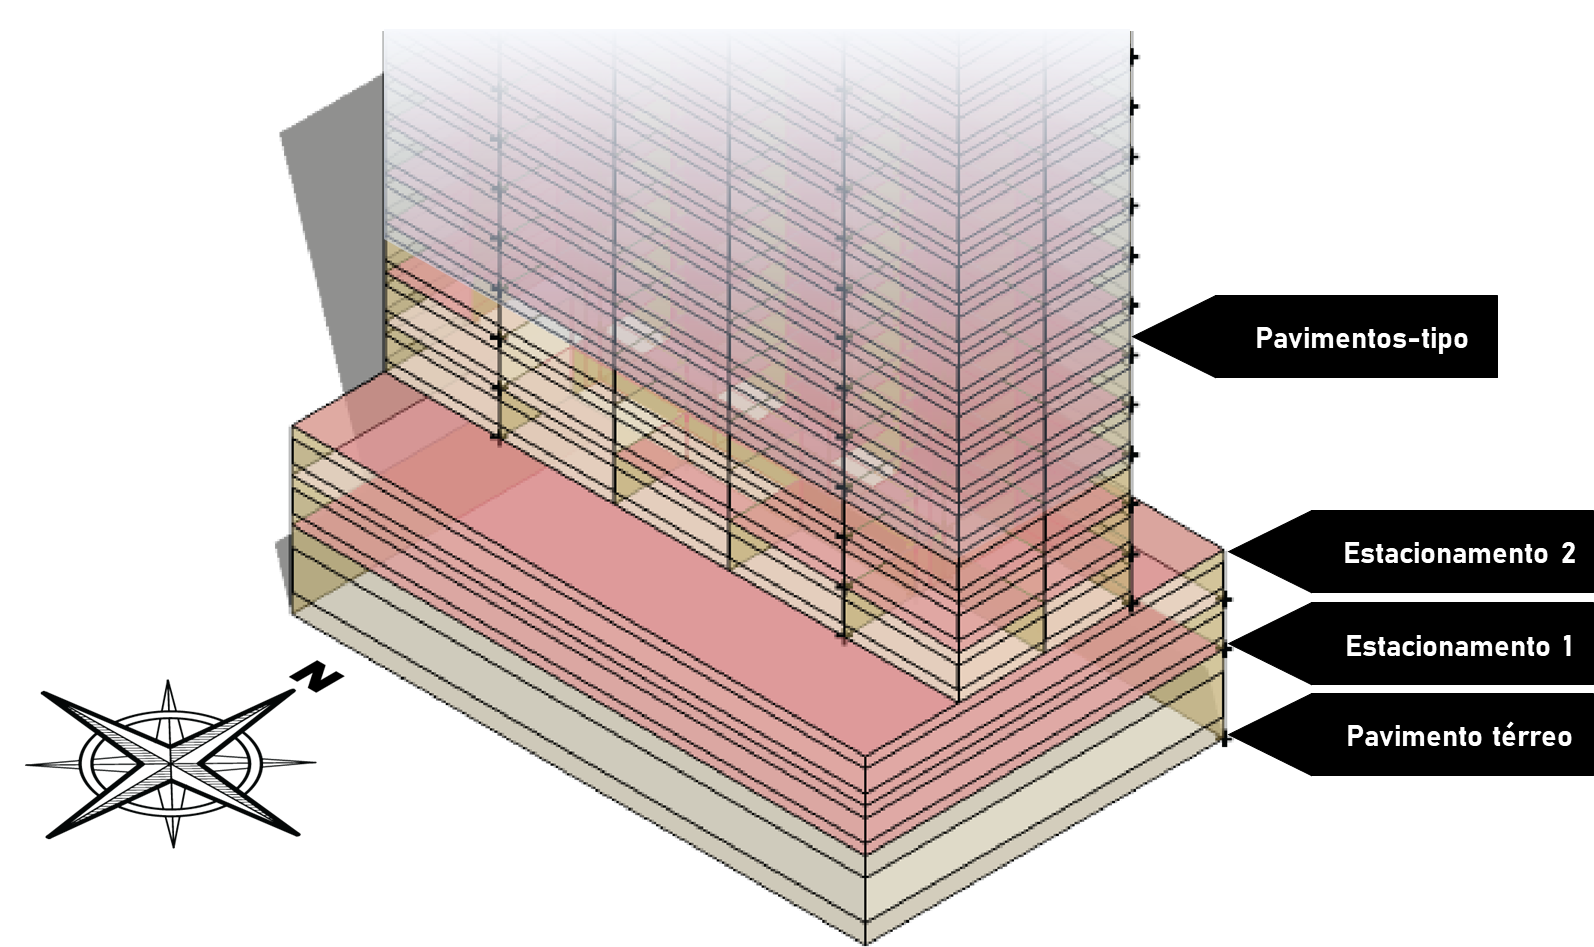
\includegraphics[width=0.6\textwidth]{figures/fig12-base_torre-1.png}
        \begin{flushleft}
            \par \small Fonte: autor (2019).
        \end{flushleft}
        \label{fig:figura12}
    \end{figure}\newline